\documentclass[10pt,a4paper]{article}
\usepackage[utf8]{inputenc}
\usepackage{amsmath}
\usepackage{amsfonts}
\usepackage{amssymb}
\usepackage{graphicx}

\usepackage{fullpage}

\title{Crystal Hypergraph Convolutional Networks}
\author{Alexander Heilman}
\begin{document}
\maketitle
\section{Introduction}
Machine learning has proven to be a computationally cost-effective and powerful predictive tool in the screening of large sets of material systems for certain material properties. Some of the most effective modern models applied to such invariant target predictions represent material systems, such as crystals or molecules, as graphs. These graphs encode physical properties in feature vectors associated with both the nodes and edges, and update or 'learn' these features via a graph neural network, described most generally with the message passing framework defined in \textit{Gilmore, et al} \cite{mpnn}. 

One problem with such graphical representations, however, is the lack of representation of larger order geometrical structure, since the constructed crystal graphs are necessarily only defined in terms of pair-wise descriptors. This may make it hard, or often, impossible, for models to distinguish between compositionally similar, but structurally unique systems. 

For example, higher order geometric information is often particularly important in the case of complex oxides, where compositions may vary subtly while structure varies substantially. 

Here, we propose the concept of \textit{crystal hypergraphs} to ail this lack of geometrical structure in the more restrictive graph representations. In a crystal hypergraph, we may define larger (than strictly pair-wise) hyperedges that correspond to higher order geometrical structures of material systems explicitly, such as triplets of neighboring atoms, first shells of neighbors or motifs, and entire unit cells. These different structures then may have different coordinate invariant features associated with them, such as angles, order parameters, and symmetry groups, respectively. Note that in that regard, crystal hypergraphs are naturally heterogeneous in their hyperedges, since there are different feature sets for different types.

Of course, the definition of a more general hypergraph representation requires the generalization of the message passing framework mentioned above. So here, we propose three possible approaches to such a generalization that handle the now-variable size of hyperedges. In a certain sense, these allow for the learning of a certain type of 'cluster-correlation expansion' by the model, where clusters of interest correspond to the hyperedges defined.

As a proof of concept, we implement the above in the first crystal hypergraph convolutional models (CHGCNN), with an eye towards extending to equivariant and different convolutional structures in future works. Even these first, basic, models give a novel application to machine learning in this field: we may compare the performance on different tasks' validation sets between models based on different hyperedge types. This allows us to investigate the importance of different order structures for these different tasks. Namely, here, we compare the performance of models based on atom, bond and triplet information against those incorporating atom, bond, and motif information (i.e. first shell hyperedges) on various predictive tasks with varying data sizes. 

Results indicate that motif level information (encoded in terms of continuous symmetry measures and local order parameters) may be sufficient, if not more informative, than triplet information (encoded as bond angles) at much less computational cost in terms of message order scaling. A point which may guide further research in the area.

The structure of this work is as follows: first, we give a brief overview of related and motivating works; then, we give an overview of crystal graph construction and message passing networks. A motivating representation problem is then identified with our definitions and the concept of crystal hypergraphs is introduced, with a particular focus on different types of hyperedges and their corresponding feature sets. Three generalized message passing are then considered, and a specific model architecture is presented. Finally, this specific architecture is used on various datasets to compare performance of different sets of hyperedge types.

\section{Related Works}
The concept of a continuous-filter convolutional operator for atomic systems, one that may adequately learn from the nuances in interatomic distance, was introduced by \textit{Schutt et al} in \cite{schnet}. The popular CGCNN \cite{cgcnn} then followed, utilizing a specific continuous-filter convolutional layer which we refer to as CGConv. 

The limitations of graphical structures in the representation of atomistic systems is well known. This limitation is addressed in several modern approaches by the inclusion of bond angle information in an auxiliary \textit{line graph} $L(G)$, derived from some graph $G$, as in M3GNet \cite{m3gnet} and ALIGNN \cite{alignn}. The edges in the derived line graph correspond to triplets in our work. This concept is further generalized by the concept of Nested Graph Networks (NGNs) to consecutive line graphs $L(L(...G)$. The edges in an $n$-line graph $L^n(G)$ then correspond to a certain subset of hyperedges of order $n+2$.

Here, we argue that an alternative approach is preferred to convolution performed on line graphs $L(G)$, since these methods require a quadratic increase in the number of additional messages with respect to the number of edges in $G$. Results suggest that a single first-shell neighborhood hyperedge for each atom provides comparable geometric resolution at much less computational cost (i.e. much fewer messages). At least, this is true for most tasks tested in this work.

\section{Crystal Graphs}
A common representation of crystalline systems in machine learning is via graphs, or, collections of nodes and binary connections between them. We may define a crystal graph $\mathcal{G}=\lbrace \mathcal{V},\mathcal{E}\rbrace$ as a set of vertices $v_i\in\mathcal{V}$, corresponding to each atom $i$, and edges $e_{ij}\in\mathcal{E}$, where edges are determined by some physical criteria.

If we take the nodes to always represent atoms in crystal graphs, a specific implementation is then left to determine by what criteria we may determine connections between atoms, or edges, from the crystalline structure. 

We also generally want to associate physical information with the objects in these graphs. This is often done by way of feature vectors. These are vectors with components describing the physical characteristics of their corresponding graph element, and which may be further 'learned' or updated through convolution.

As such, crystal graphs are essentially defined by two (potentially task dependent) concerns: the criteria by which to derive edges from; and the features we choose to associate with the atoms and edges, which encode all of the physical information of the system. Below, we give the usual approaches for the construction of crystal graphs in terms of these concerns. Note, however, that while this section is meant to exemplify other works' approaches, we also use the following in the first step of crystal hypergraph generation.

\subsection{Edge Criteria}
Perhaps the simplest (and most often applied) criteria for the formation of edges between atoms is a combination of a maximum distance cutoff $r_{max}$ and a maximum number of neighbors for each node $N_{max}$. That is, for each atom, we construct edges for up to $N_{max}$-th closest neighbors in the crystalline structure within a shell of radius $r_{max}$.

\begin{center}
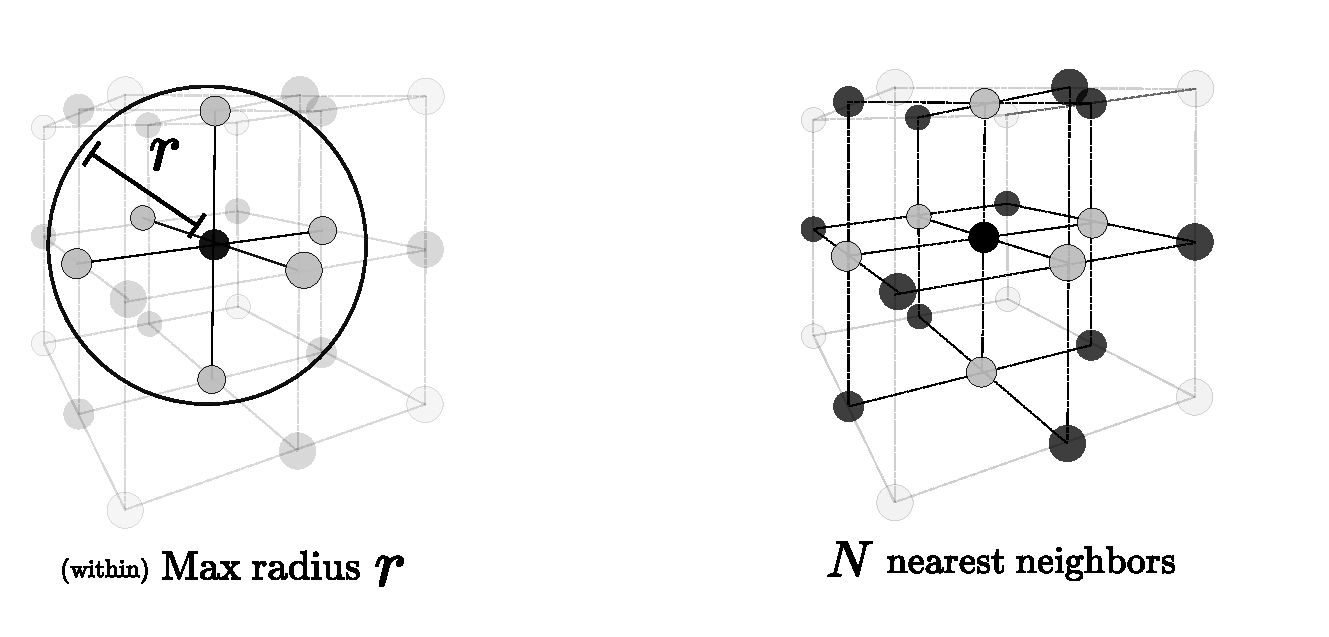
\includegraphics[scale=0.45]{ex_bondcriteria.pdf}
\end{center}
While other criteria may also be utilized, such as face-sharing in Voronoii Tesselations, and scaled maximum distance cutoffs based on nearest neighbor distances, these more advanced criteria are generally more computationally expensive in the data processing stage. Alternatively, most models \cite{cgcnn,alignn,megnet} adopt the more basic criteria of maximum numbers of neighbors within cutoff shells, and adopt some continuous-filter convolutional function that can learn which connections are more important for the task at hand.

Often, the maximum number of neighbors considered is chosen to be $12$, however recent tests in coNGN \cite{congn} suggest even this may be too restrictive, and show that a maximum set as large as 24 may improve performance.

%As a maximum distance cutoff, since we focus primarily on crystalline structures here, we consider $6$ \AA $ $  to be sufficient.


\subsection{Crystal Graph Features}
With the means of edge determination settled, we now wish to incorporate more physical information with this derived graph representation. 


Node features encode all of the atomic information of the sites they describe. Two usual techniques include: explicitly engineered feature vectors (as in \cite{cgcnn}); and the learning of encodings for atomic sites based only on their atomic number (as in \cite{megnet}), beginning with some random initialization.


Note that we could also, in principle, include an atomic position in the node features. However, this would require a special treatment of such information through convolution if we wished to maintain an \textit{invariant} representation up to choice of coordinate system. As such, often only coordinate system (or more specifically, Euclidean group) invariant features are included in crystal graph representations. This restriction to invariant features also precludes any inclusion of unit vector orientation in edge features which are discussed below.

Edge features are further limited, to a certain extent, by their determination criteria. That is, if one determines edges based solely on their distance, and not at all on ionic or covalent structures, it is hard to justify the inclusion of specific bonding information in the corresponding edge features. 

For edges determined exclusively by distance and a desired coordinate system invariance in edge features then, edge features are often derived exclusively from their distance. This distance is often expanded in dimensionality using some Radial Basis Function (RBF: $\mathbb{R}\rightarrow\mathbb{R}^{d_{RBF}}$ where $d_{RBF}$ is the dimensionality of the radial basis function), such as a Gaussian or Bessel expansion.


\begin{figure}

\begin{center}
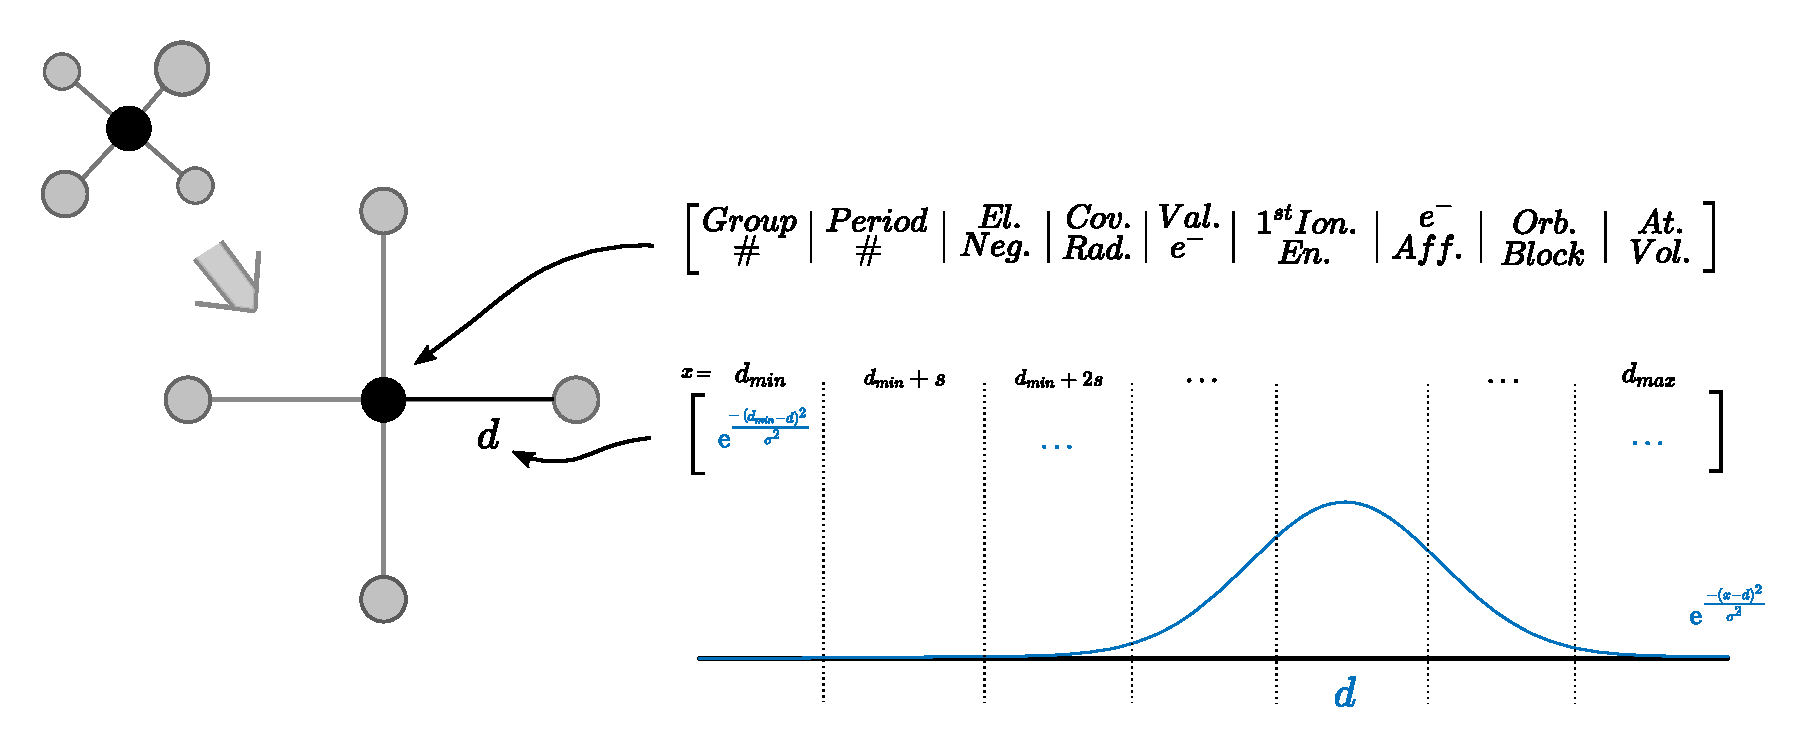
\includegraphics[scale=0.5]{crystal_graph_feat.pdf}
\end{center}

\caption{Schematic for a simple CGCNN-like graph encoding of some basic atomic structure. Note that the atomic properties are generally expanded by some one-hot encoding or RBF expansion and then concatenated. The edge feature here then is given, as an example, in terms of a Gaussian expansion of $d$, where $d$ is the relevant interatomic spacing.}
\end{figure}
These features are typical to modern machine learning models, with some notable exceptions and advancements (specifically those utilizing line graphs) to be considered later. We also note some limitations with these representations in the section after that which follows.

\subsection{Crystal Graph Convolution}
Crystal graphs are usually constructed for their sole use in some graph convolutional neural network. Perhaps the most general framework in which we may define graph convolution is the message passing framework, defined by Gilmore \cite{mpnn}.
A message passing network updates nodes based on 'messages' generated by the features of, and passed through, neighboring nodes (that is, nodes sharing an edge). Gilmore defines the message passing framework in terms of three functions: $M$, the message forming function; $U$, the node update function; and $R$, the readout function. These three functions act on graph representations as follows:

\begin{gather*}
m_i^{t+1}=\sum_{n_j\in \mathcal{N}(i)} M_t(n_i^{t},e_{ij},n_j^t )\\
n_i^{t+1}=U_t(n_i^t,m_i^{t+1})\\
\hat{y}=R(\lbrace n_v^T\rbrace)
\end{gather*}
Where for each pair of connected nodes (or edge), a message is formed from each node's representation $n_i^t,n_j^t$, of layer $t$, and the connecting edge's feature $e_{ij}$. These  node representations of layer $t$ are updated to their $t+1$-th layer representation by update function $U_t$ of layer $t$, which takes as input the set of messages for each node, and the nodes current representation. At the final layer $T$, the readout function $R$ then predicts the target value from the updated node representations.


Message passing networks acting on crystal graphs have several advantages: message passing networks enjoy invariance under permutation of node indices; and, further, if the encoded features are coordinate system invariant, the output of the network is itself coordinate system invariant.


\subsection{Disadvantages of Crystal Graphs}
Perhaps the most poignant problem with our construction above though is the lack of higher-order geometrical information, i.e. local geometrical environments of atoms (that is, motifs) and global crystalline symmetries.

As a simple example of the low resolution manifest in crystal graphs, consider two atomic systems below: one with a local cubic symmetry, and another with a square anti-prism local environment; but both with the same bonding atoms. 
\begin{center}
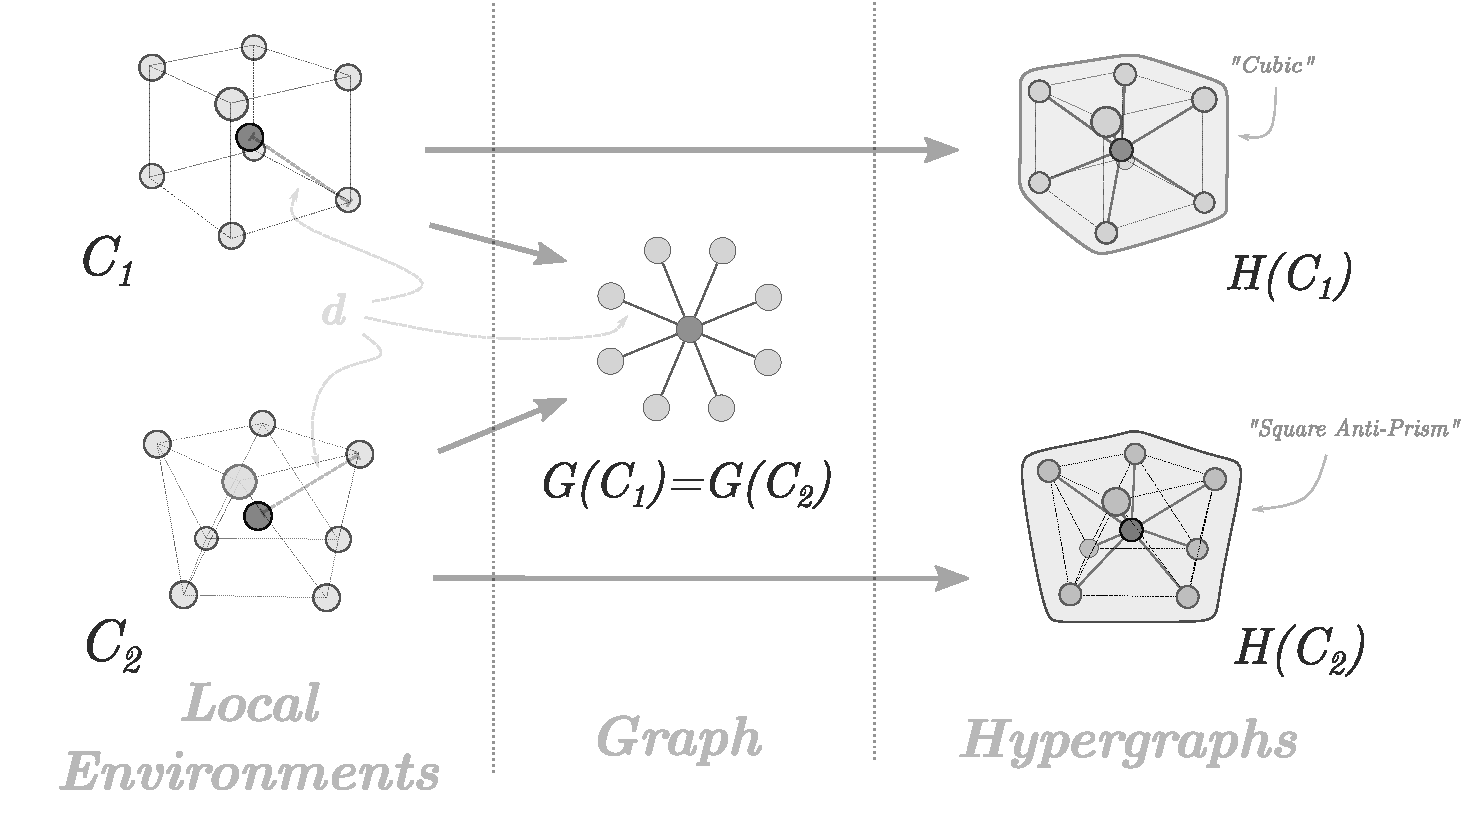
\includegraphics[scale=0.63]{graph2hgraph_tall_revise.pdf}
\end{center}
In the above constructions, both would map to the exact same crystal graph, but could be easily be distinguished with an additional descriptor describing the local geometry of each's central atom.


\section{Crystal Hypergraphs}
The extension proposed here solves the above problems by allowing for the explicit incorporation of this higher-order geometrical information in the form of hyperedges, which can be used to represent these higher-order structures explicitly.



A crystal hypergraph $\mathcal{H}=\lbrace\mathcal{V}, \mathit{H} \rbrace$ is a collection of nodes $v_i\in \mathcal{V}$ and hyperedges $h_j\in \mathit{H}$ (containing an arbitrary number of nodes), where the hyperedges are most generally heterogeneous (that is, we may wish to describe different types of structures in the same hypergraph). These objects further have associated feature vectors encoding relevant physical information, which we also refer to as $v$ and $h$.

For the purpose of modeling material systems, we need first consider what different order structures are most important in their representation. Of course, atomic and bond level information is particularly important. However, higher order structures may also be of interest, such as: triplets of atoms, local environments of atoms (motifs in oxides), and entire crystalline unit cells of atoms.

Each of the aforementioned structures also has a natural set of distinct, coordinate-system invariant features that may be associated with them. At the triplet level (where two bonds share some common node), there is always a corresponding angle. At the motif level, order parameters \cite{orderparam1, orderparam2} or continuous symmetry measures \cite{csm_polyhedra, chemenv} may be used to describe 3D coordination environments quantitatively. And, at the unit cell level, we have the underlying crystal structure itself.
%\begin{center}
%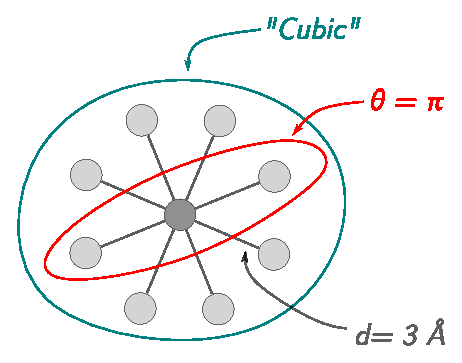
\includegraphics[scale=0.7]{hypergraph_6.pdf}
%\end{center}


These different order structures may all be represented in a single crystal hypergraph. Below, we discuss the generation of, and association of features with, all of the above mentioned structures in crystalline solids. 

\begin{center}
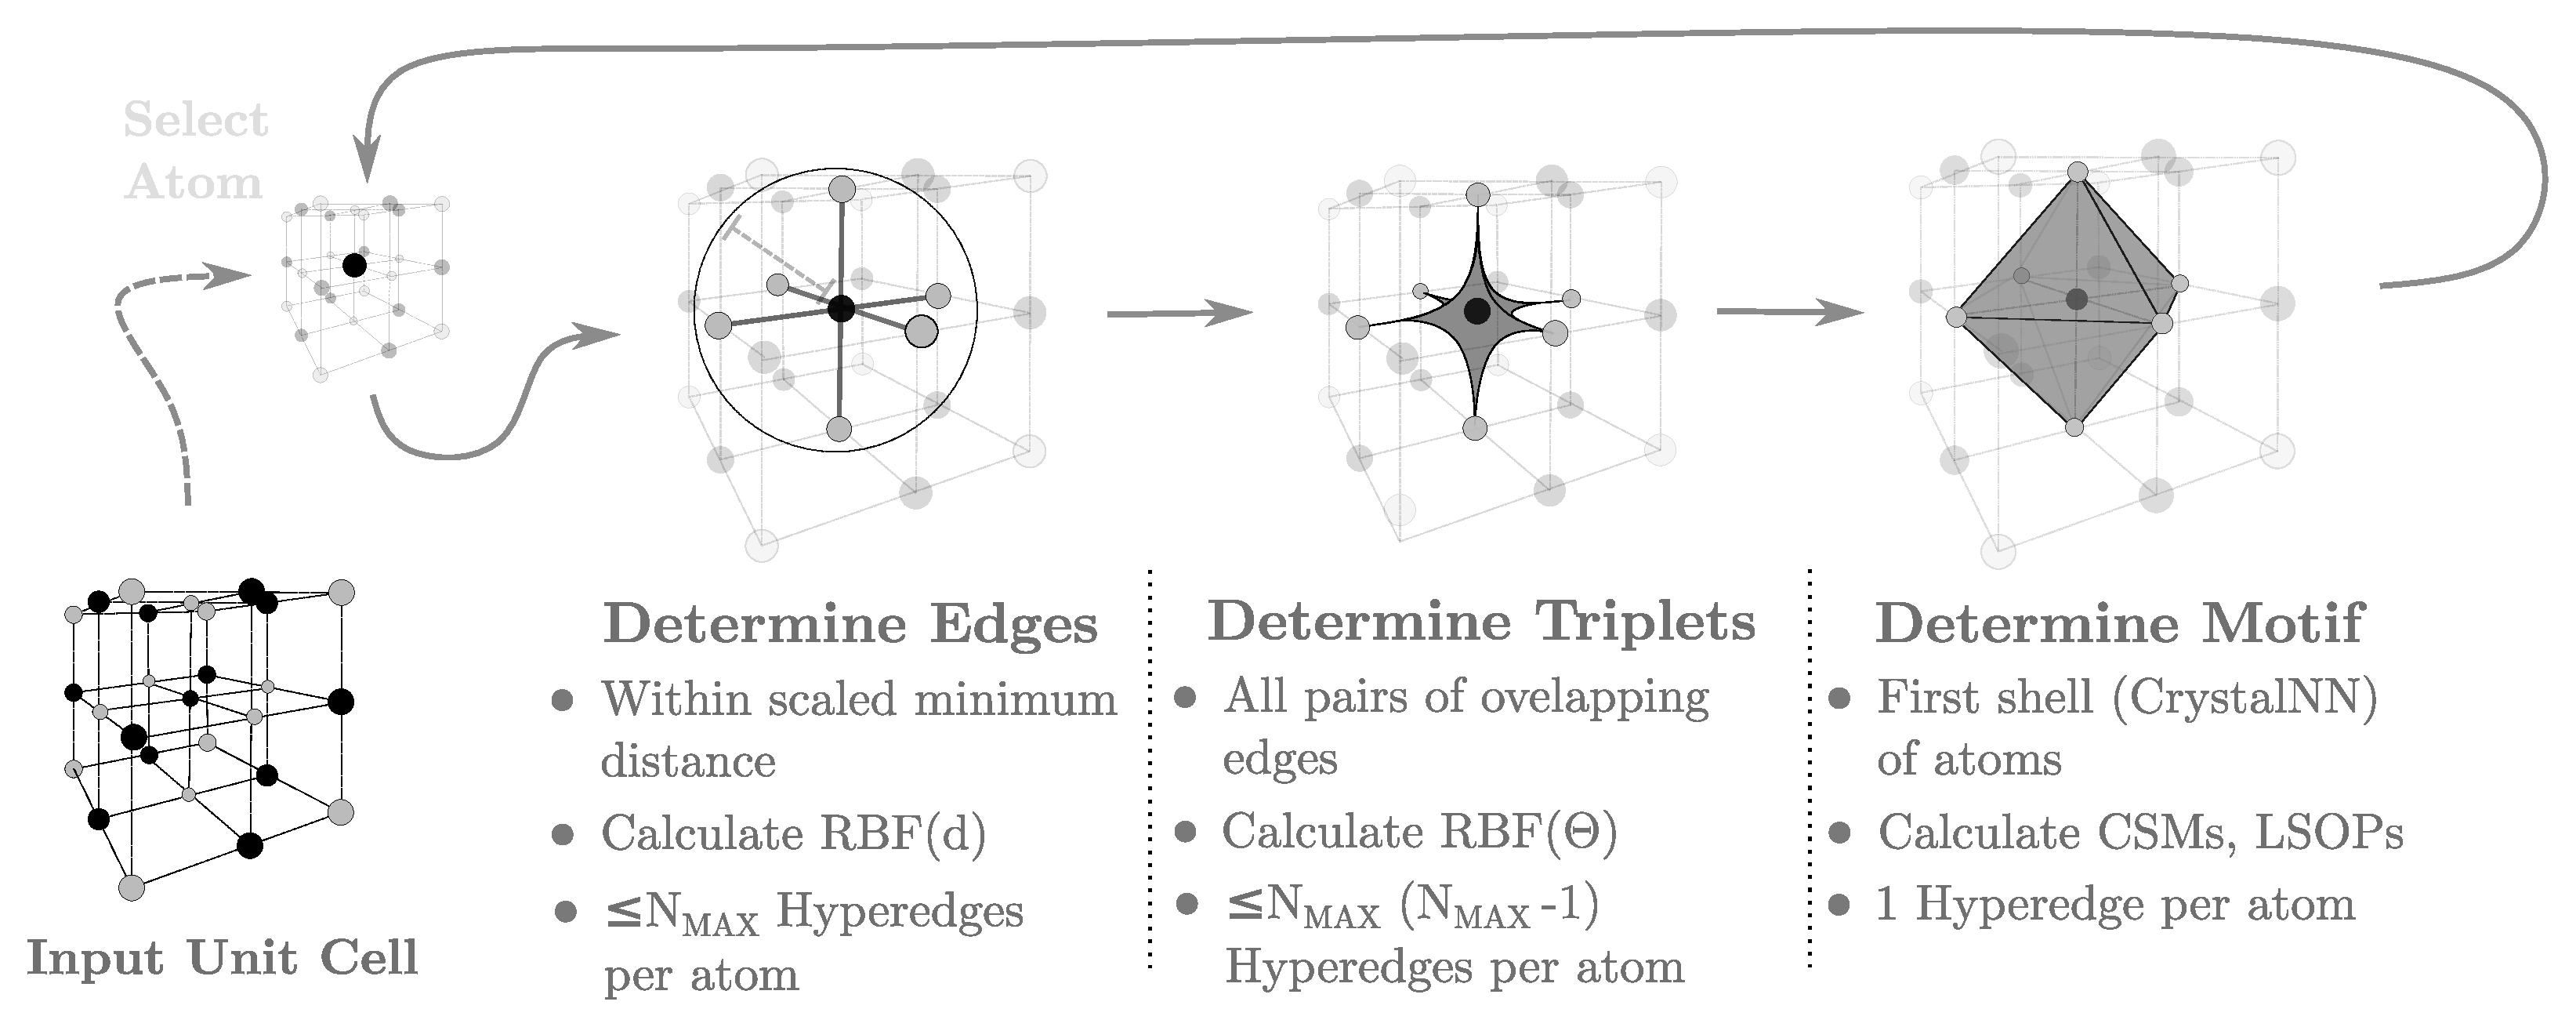
\includegraphics[scale=0.27]{crystal_hgraph_ex.pdf}
\end{center}

\subsection{Bond Edges}
Bonds, or pair-wise atomic connections, may be made in parallel to the approach detailed in the crystal graph section above. In the results below, for instance, we choose edges from a maximum number of neighbors $N_{max}=12$ found within a shell of radius $r_{max}=6\AA$. 

The feature associated with such edges is a Gaussian expansion of the distance, with a range from 0 to 6 Angstrom and a dimensionality of 40.

\subsection{Triplet Hyperedges}
Triplet hyperedges are then formed from the set of bonds, where for each set of bonds connected by one node, a triplet hyperedge is formed.

The feature of these triplet hyperedges is also a Gaussian expansion of the angle formed by the unit vectors of the two bonds.

\subsubsection{Comparison to Line Graph}
A more usual approach for the incorporation of bond angle information is via the construction of a line graph, as in \cite{alignn, m3gnet}. 
\begin{center}
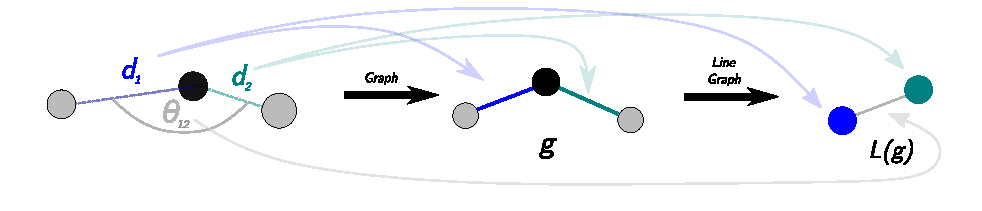
\includegraphics[scale=0.7]{line_graph_ex.pdf}
\end{center}
These models generally first update the edge features of the crystal graph $\mathcal{G}$ by first applying some graph convolutional operator to the line graph $L(\mathcal{G})$ with angles encoded in  $L(\mathcal{G})$'s initial edge features.

Our argument against such representation schemes here is that the order of messages grows combinatorically for derived line graphs as $\mathcal{O}(nm^2)$, where $n$ is the number of nodes and $m$ is the average number of edges per node in $\mathcal{G}$.

Here, we incorporate a similar level of higher order geometrical structure instead in a local environment, or 'motif', hyperedge (defined below). Note that these include only an extra number of messages on the order $\mathcal{O}(mn)$ if each node in a motif gets a message, or on the order $\mathcal{O}(n)$ if only center nodes are updated by it's own motif hyperedge(s).

\begin{center}
%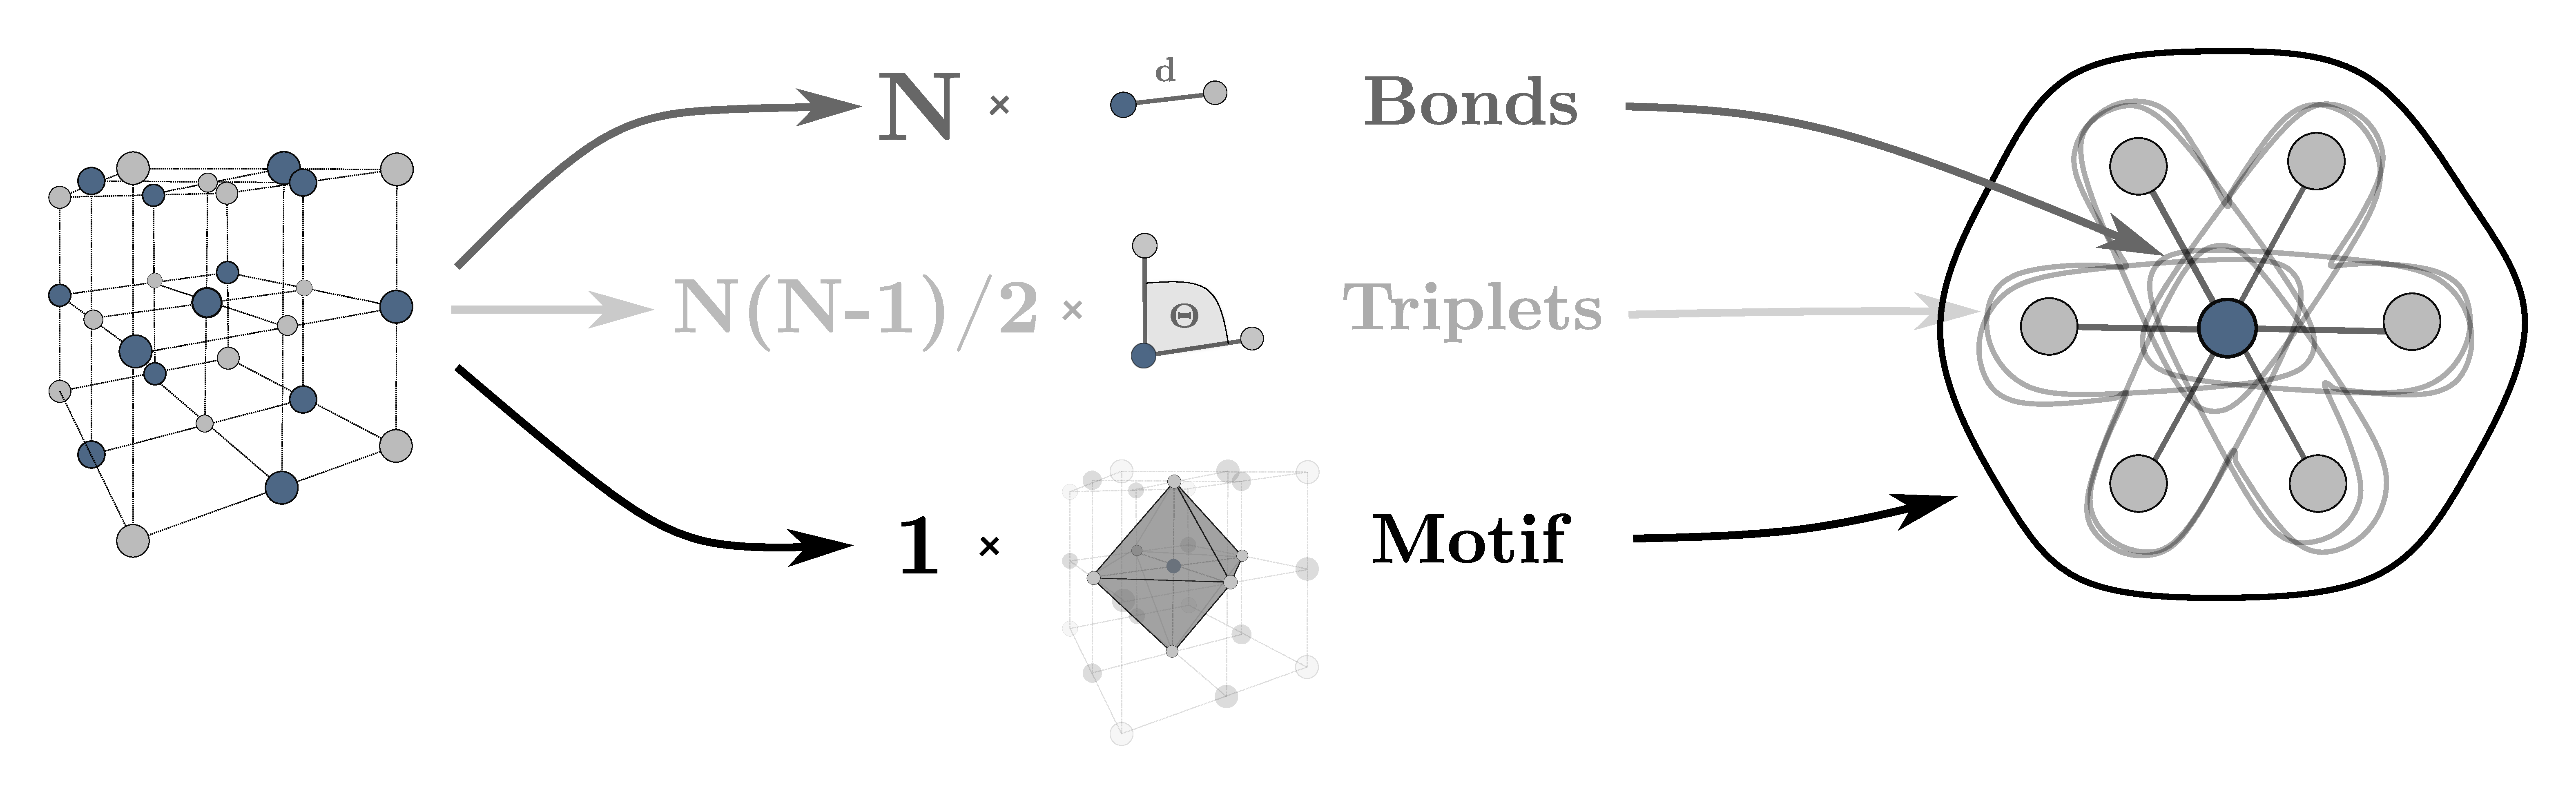
\includegraphics[scale=0.15]{revamp.pdf}

%OR

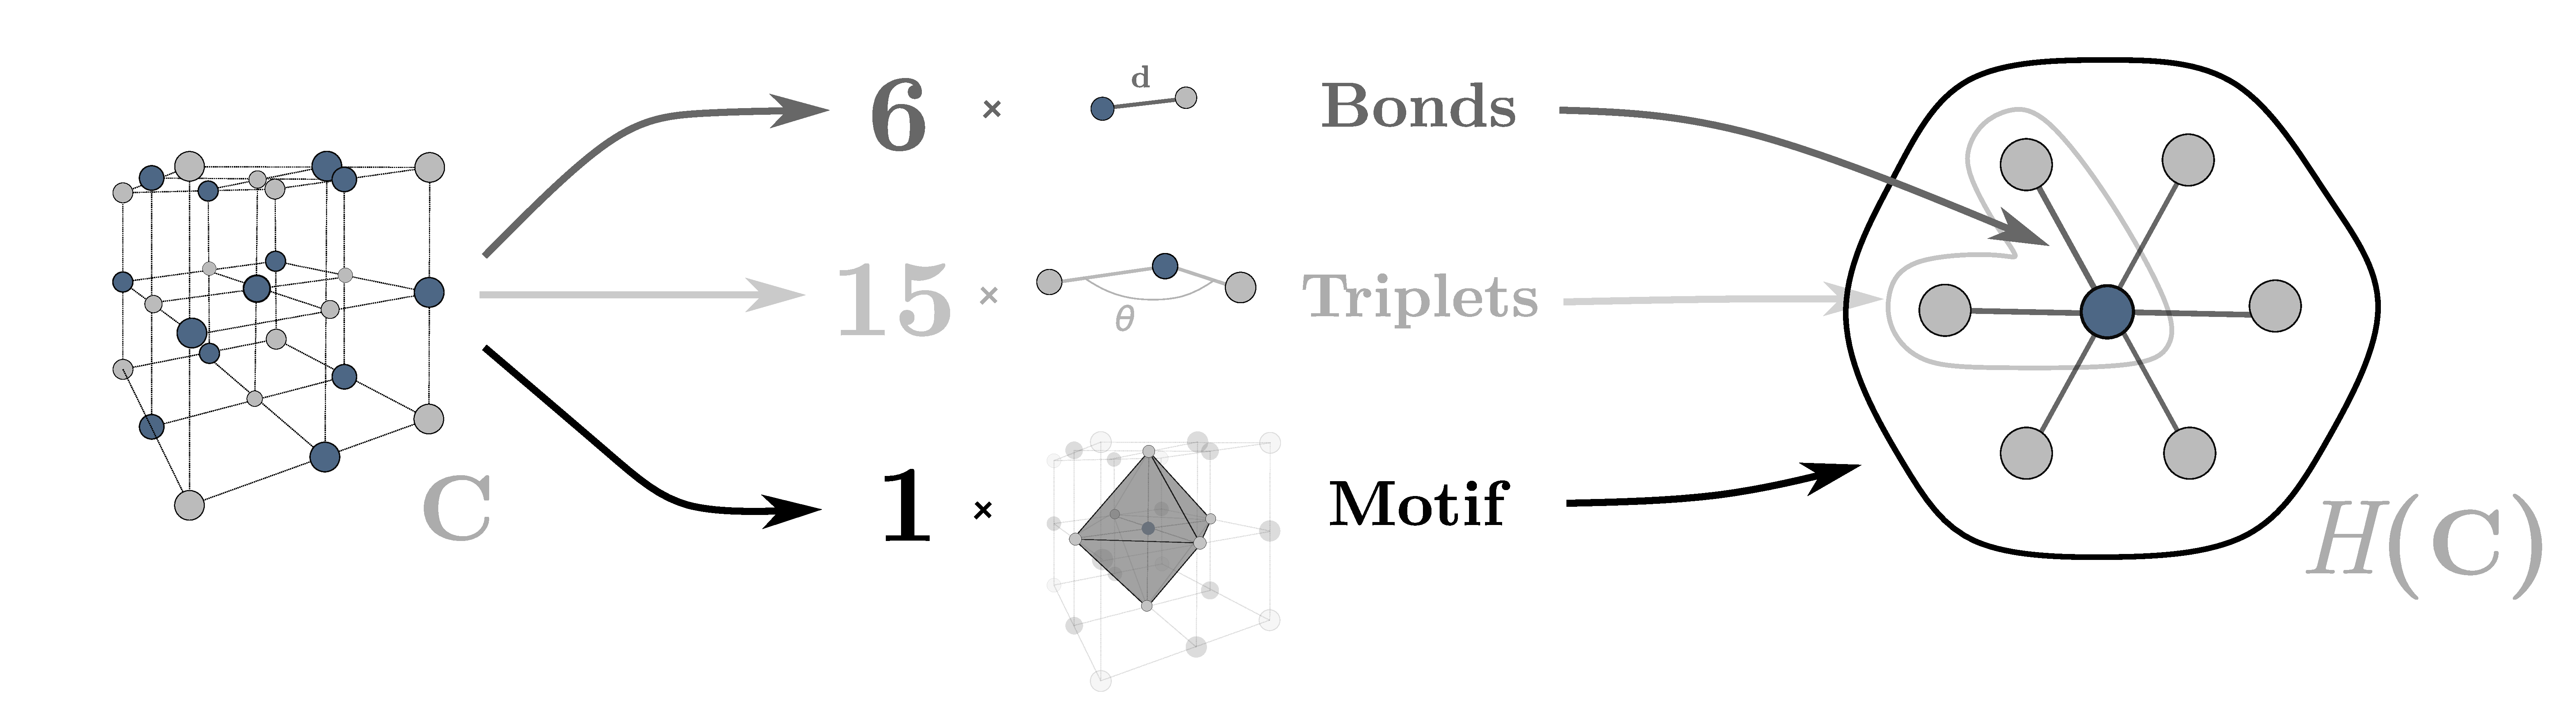
\includegraphics[scale=0.13]{revamp2.pdf}

\end{center}


\subsection{Motif Hyperedges}
Motif determination may be achieved by a wide range of functions, and is akin to an algorithmic determination of coordination number. Here, we use the method implemented as CrystalNN in pymatgen. Note this is a much stricter algorithm than that used to determine edges and triplets.


The features of these motifs include Zimmerman's 35 local structure order parameters \cite{orderparam1,orderparam2}, and continuous symmetry measures \cite{csm_polyhedra} (e.g. 'distance to a perfect shape') calculated for 59 common coordination environments. Essentially, these are both just sets of quantitative measures designed to describe 3D physical shape.

%\subsection{Cell Hyperedges}
%Cells of the overall atomic structure can also be given one master hyperedge with a feature encoding the underlying crystalline structure or symmetry group. This master hyperedge feature may alternatively be learned through convolution and then used as a crystal-level feature vector for predictive tasks.

%These 'unit' cell hyperedges allow for the explicit inclusion of global crystalline structure properties, i.e. point group information. The definition of the cell hyperedge is perhaps somewhat arbitrary, in that a single primitive cell may suffice as well as a larger conventional cell. The approach taken in this work was to simply include all the nodes within some global hyperedge, regardless of the input size. This cell-level edge had a feature embedding based on the crystal's point group.

\section{Crystal Hypergraph Convolution}

We now must consider a message passing framework analagous to \textit{Gilmore, et al} \cite{mpnn} but applying to hypergraph structures. That is, we now have:

\begin{align*}
m_v^{t+1}&=\sum_{h_j\in \mathcal{N}(v)} M_t(n_v^{t},h_j^{t},\lbrace n_w^t \vert n_w \in h_j \rbrace),\\
n_v^{t+1}&=U_t(n_v^t,m_v^{t+1}),\\
\hat{y}&=R(\lbrace n_v^T\rbrace),
\end{align*}
so that each node is still updated according to layer-wise update function $U_t$, aggregating messages $m^{t+1}$ formed from origin node features, hyperedge features $h_j$, and hyperedge neighborhood features $n_w \in h_j$, in analogy to the graph-based MPNN approach. This updating occurs node-wise and then after $T$ layers, some readout function $R$ is again used to output the corresponding predicted value $\hat{y}$, which utilizes the set of learned node features.


%where $m_v^{t+1}$ is the message formed for node $v$ in the $(t+1)$-th layer; $M_t$ is the message function; $n_v^t$ is the node representation; $h_j^t$ is the representation of the $j-$th hyperedge feature with a neighborhood contain node $n_v$, which compose the 'neighborhood' of node $v$, $\mathcal{N}(v)$; $U_t$ is the representation update function; and $R$ then is the readout function giving the predicted value $\hat{y}$.
  
The biggest difference here is that we now need a message forming function $M_i$ that accounts for a set of node features $\lbrace n_w^t \vert n_w \in h_j \rbrace$, that may vary in size between different hyperedges (even of the same type). This stands in opposition to the case of regular edges, where we are assured a fixed size of two nodes per edge. 

One approach would be to fix the dimensionality of each type of hyperedge, or have a different convolutional operator for each different size hyperedge (as is effectively the approach taken in line graph networks). Here, however, we wish to maintain generality in edge size so we need not fix hyperedge orders for different types, as motifs with different coordination numbers, or different size unit cells, may be described by common sets of features.

Note that we may also wish to update hyperedge representations of one type according to other hyperedges of the same or other types. As an example, we may desire the two bonds forming a triplet to be updated from messages based on the angle they form. Or, we may hope to update a motif's representation based upon the unit cell it resides in. 

These connections between the same or different orders of hyperedge may be defined based upon inclusion and/or contact. In the case of the bond-triplet-bond interaction, we may determine the relationship between these hyperedges by forming messages for bonds included in triplets. Furthermore, we may care to relate triplets that are touching each other, or mutually contain one or more nodes.

Of course, there should be different message and update functions for each different order structure (bonds, triplets, motifs, etc.) with different features. This is accounted for by treating the data as a heterogeneous graph, with different hyperedge types. Below, we consider three strategies that allow us to apply our convolutional operator to hyperedges of arbitrary size.


\subsection{Three Possible Approaches to Hyperedge Convolution}

Three general approaches for message passing that account for this multi-order nature and which can be used to incorporate inter-order hyperedge message passing have been considered in this work: \textbf{1.} the construction of a hyperedge relatives graph, upon which regular graph convolution may be applied; \textbf{2.} total exchange hyperedge message convolution, which completely generalizes the CGCNN \cite{cgcnn} and ALIGNN \cite{alignn} models to hypergraphs; and \textbf{3.} neighborhood aggregation, which balances performance of the former approach by forming a single neighborhood feature for each hyperedge.

Each approach has a different computational cost in terms of total number of messages, along with a potentially different practical definition of a hypergraph. These considerations are presented below, with a specific convolutional structure and empirical results on common test datasets then presented after.

%Note also that through testing, a guiding principle was learned for hyperedge messages: each order of hyperedges should contribute the same number of messages to each node. That is, each node should be updated by some global, fixed number of messages for that order of hyperedges.

\subsubsection{Hyperedge Dual Graph}
We may define a dual graph $\mathcal{D}(h)$ to a hypergraph $h$ to be a graph in which nodes represent the hyperedges of the hypergraph, and connections represent the overlap of respective hyperedge neighborhoods. 

In the case of a crystal hypergraph with heterogeneous hyperedges, this dual graph is a graph with heterogeneous nodes. We term this heterogeneous dual graph of a crystal hypergraph the relatives graph for simplicity. 
Note that atomic features may be included by adding a singleton hyperedge for each node.

The definition of the relatives graph allows us to perform the usual methods of graph convolution on hyperedge features. And thus, requires we only define an edge index describing the connection between different hyperedges and nodes.

\begin{center}
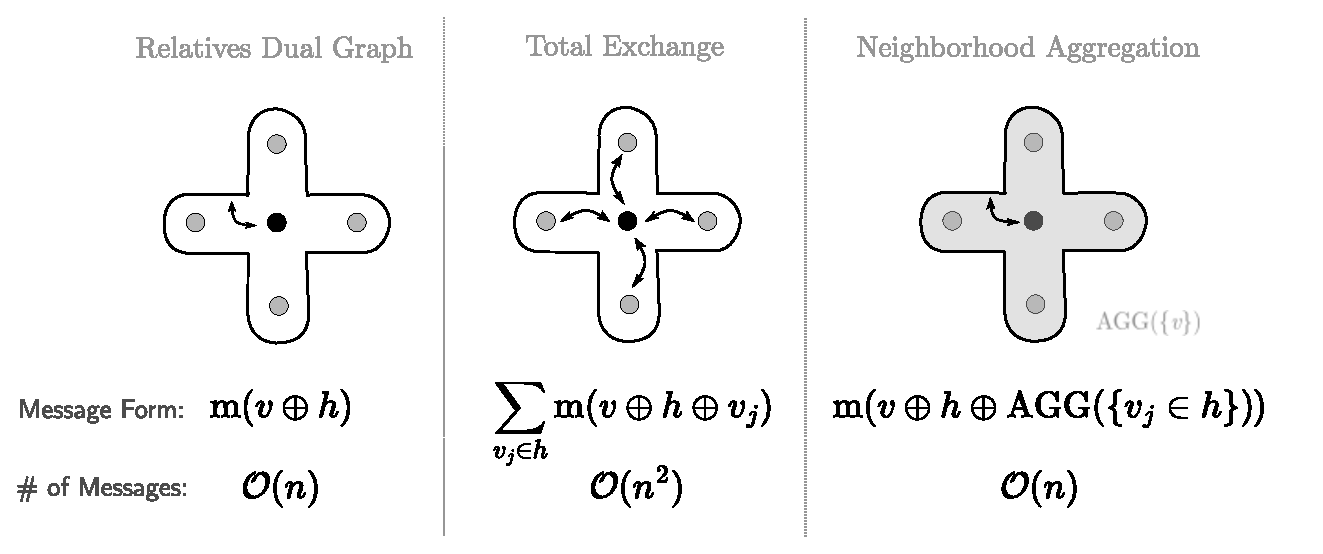
\includegraphics[scale=.75]{HMPNN.pdf}
\end{center}
However, this approach lacks the interaction of neighboring features in convolution via the connecting hyperedge. That is, without a clear definition of the edge attribute, messages are generally of the form below:
$$
m_v^{t} = \sum_{h_j\in \mathcal{N}(v)}M_t(n_v^{t},h_j^{t})
$$
in which we simply discard the neighborhood of other node features contained in the hyperedge.

Computationally, this approach has a total number of messages that scales linearly with average hyperedge size, since each hyperedge only contributes one message to each node it contains.
Accounting only for node-hyperedge connections in a relatives graph derived from a hypergraph with $m$ hyperedges of average order $n$, the total number of messages per convolution will scale as $\mathcal{O}(nm)$.
 
\subsubsection{Total Exchange}
Of course, we may wish to incorporate the neighboring features of some representation via their connecting hyperedge. This may be accomplished by simply forming a message for every pair of connected representations along with their connecting hyperedge's representation.
$$
m_v^{t} = \sum_{h_j\in \mathcal{N}(v)} \sum_{n_w \in h_j } M_t(n_v^{t},h_j^{t}, n_w^t),
$$
Note that this method completely generalizes previous approaches based on line graph convolution, or nested graph networks.

Here, though, we've introduced a new summation which may drastically increase the number of messages for larger hyperedges. If each hyperedge contains an average of $n$ nodes, and there are $m$ hyperedges in some hypergraph, the total number of messages exchanged per node-wise convolution will scale as $\mathcal{O}(n^2m)$.

%This approach also requires a different practical definition of the hypergraph.  Instead of a two dimensional index set, we now define a three dimensional index set, relating the origin node, the connecting hyperedge, and the connected node.

\subsubsection{Neighborhood Aggregation}
Since the number of messages will scale tremendously with larger hyperedges in the framework described above, we may seek a way to incorporate the neighborhood of features of a hyperedge into a single message.

In this case, we may essentially form a 'neighborhood feature' representative of all a hyperedge's contained nodes. Typical aggregation methods may be used and trained to perform this neighborhood feature generation. Here then, we deal with message functions of the form:
$$
m_v^{t+1}=\sum_{h_j\in \mathcal{N}(v)} M_t(n_v^{t},h_j^{t},\text{AGG}\big(\lbrace n_w^t \vert n_w \in h_j \rbrace\big)
$$
This results in a number of node-wise messages that scales linearly with the average size of hyperedges, so that we now have a relationship of order $\mathcal{O}(nm)$ again, while still incorporating the features of neighboring nodes.

This approach also reduces the definition of the hypergraph back to a two dimensional, though now hyperedge, index set; where the first index is the node contained and the second index is the containing hyperedge (as in \cite{hypergraphconv}).




\subsection{Example Model Architecture}
Node and hyperedge features were first passed into a linear embedding layer (with no activation function), these were then updated via CHGConv layers applied in alternating order to bond and motif features (bond, motif, bond, motif). The learned node features were then mean pooled to form a crystal vector, which was passed to a fully connected layer and then projected down to a one-dimensional (scalar) output for regression. In the case of classification tasks, the fully connected layer, after mean pooling, utilized a dropout mechanism and output a probability distribution of classes via a softmax activation function.

\begin{center}
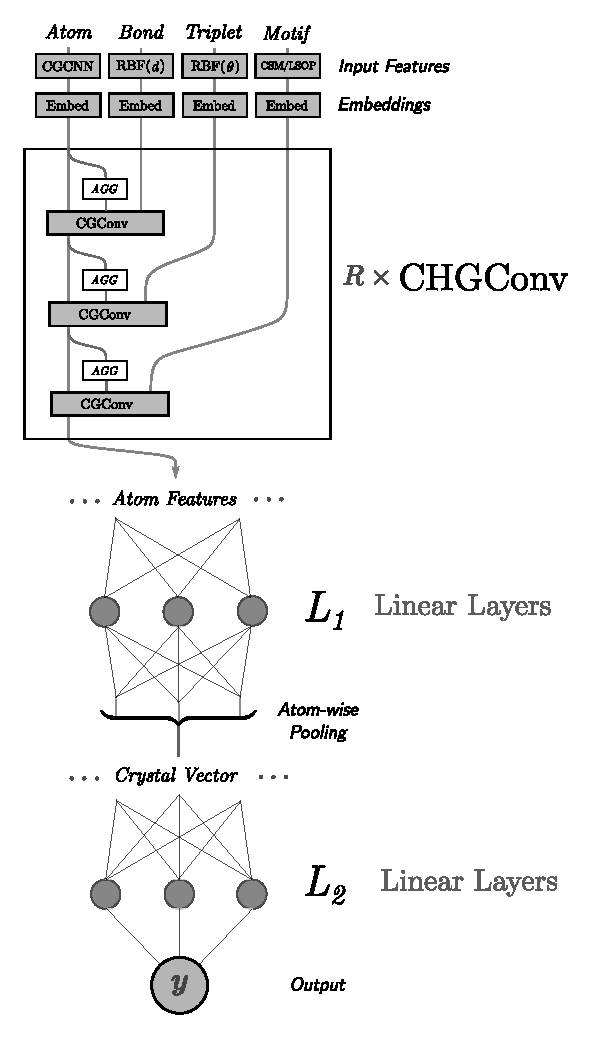
\includegraphics[scale=.75]{arch.pdf}
\end{center}


\section{Training and Results}
Even with a basic convolutional structure (i.e. currently bad results overall), crystal hypergraph networks provide a unique opportunity to investigate the importance of different order correlations for different physical properties of the same systems. That is, by comparing validation results for different types of hyperedges, one may probe the importance of certain structures (i.e. motifs vs. triplets) by comparing such predictive performance of these different order models.

As such, a basic continuous filter hypergraph convolution is adopted here, with the specific details given in \ref{chgconv}; leaving performance improvements to be sought in different convolutional structures in future works. 

Thus, we here focus on the comparative performance of models with different types of hyperedges on a common set of targets. Namely, we test models with and without bond, triplet, and motif level hyperedges on several invariant targets including formation energy, band gap, dielectric constants and elastic constants from both Materials Project (Table \ref{fig:mp_table}) at large, and the more curated MatBench datasets (Table \ref{fig:matbench_table}).


 
\begin{figure}\label{fig:matbench_table}\small
\begin{tabular}{c|ccccc}
 & Phonons  & Refractive Indices& Perovskites  & Log$_{10}$($G_{vrh}$) & Log$_{10}$($K_{vrh}$) \\
 & (\textit{1,265}) &  (\textit{4,764}) & (\textit{18,829}) & (\textit{10,987}) & (\textit{10,987}) \\
 & MAE (cm$^{-1}$) & MAE & MAE (eV/Atom)& MAE (Log$_{10}$GPa)& MAE (Log$_{10}$GPa)  \\
\hline
Bond-only & 84.1& 0.497 & 0.0584 & 0.099 & 0.083\\
Triplet-only & 71.3& 0.520 & 0.0566 & 0.094 & 0.073 \\
Motif-only & 77.6& \textbf{0.485} & 0.0611 & 0.103 & 0.077\\
Bond \& Triplet & 69.2& 0.550 & 0.0550 & \textbf{0.088}& \textbf{0.071} \\
Bond \& Motif & \textbf{64.5}& 0.510 & \textbf{0.0488}&0.095 & 0.073\\
\end{tabular}
\caption{Validation dataset results for several MatBench target sets, note that the italicized numbers next to the target name correspond to the total size of each dataset. Best results are indicated in bold.}
\end{figure}

\begin{figure}\label{fig:mp_table}
\begin{tabular}{c|ccc}
Hyperedge & Form. Energy & Band Gap & Metal/Non-metal \\
Types & Best MAE (eV/Atom) & Best MAE (eV) & Best Accuracy \\
\hline
Bond-only & 0.177 & 0.315 & .837 \\
Motif-only &  0.088 & 0.387 & .853\\
Bond \& Motif &  \textbf{0.074} & \textbf{0.301 } & \textbf{.860}\\
\end{tabular}
\caption{Validation dataset results for several Materials Project target sets. Here, each dataset included a total of 152,605 materials. Best results are indicated in bold.}
\end{figure}


%\section{Conclusion}
%Graphs are a relatively restrictive representation system for crystal structures, which have clear structures beyond just pair-wise interaction. Especially in the manner they are most usually constructed, crystal graphs are often of low geometrical resolution; in that related but distinct structures may map to the same crystal graph.

%Other modern works often address this lack of geometrical resolution by auxiliary, iteratively derived, line graphs, in which angles of triplets, dihedrals, etc. may be associated as features. One problem with such approaches, however, is the quadratic increase in graph size with each iterative construction.

%The primary argument of this paper then is that hypergraphs are a more natural representation of crystal structures that allow us to incorporate this lost geometrical information for different substructures of our choice.  Hypergraphs allow us to explicitly incorporate coordinate invariant features with higher order structures, such as triplets and motifs, as feature vectors associated with a heterogeneous hyperedge set.

%The introduction of a new representation scheme requires a generalization of previous convolutional methods, most generally described by the MPNN framework. Here, we considered three approaches to generalize the message passing framework to variable order hyperedges. These allow us to perform supervised learning tasks on crystal hypergraphs.

%A basic crystal hypergraph convolutional neural network (CHGCNN) was implemented and tested with and without bond and motif hyperedges. These results were compared for several different material property target sets of various sizes.

%Structural tasks seemed to benefit greatly from the inclusion of explicit geometrical information in the way of motif-level features. However, electronic tasks seemed to benefit much less from motif-level information, sometimes performing better with only bond-type edges. These tendencies seemed to be particularly prevalent in smaller datasets though, suggesting datasize scaling effects may also be contribute to this trend.

Perhaps the strongest point to be made in regards to the results is that for most tasks, motif information contributes to comparable or better performance than triplet-level results. This is at much less computational cost in terms of the total number of messages exchange through convolution. 

Future works may investigate more powerful hypergraph convolutional operators for improved performance. Other order structures (beyond motif-level) or hyperedges representing defects may also be of interest for future works. The inclusion of equivariant features and equivariant convolution may also be desired for certain tasks on hypergraphs.



\nocite{*}

\bibliographystyle{annotate}
\bibliography{chgcnn.bib}

\appendix

\section{Motif Determination}
Motifs are determined according to criteria similar to that used in bond determination. Namely, interatomic distance, Voronoii tesselations, and solid-angles of Voronoii faces are still relevant. Despite this similarity in potential criteria, testing showed more restrictive approaches to motif determination resulted in better performance on validation sets. This stands in contrast to edge determination, where the continuous order convolution operators may be used to 'pick' the more important bonds from a large, loosely defined set of bonds, by the corresponding distance feature.

Several different schemes were tested for a single task (band gap) with a relatively large amount of samples (150,000) and compared. First, the same criteria as bonds was applied (that is, all within a certain radius, up to a maximum number of neighbors), which performed worst. Second, a scaled minimum radius cutoff was applied, where for each site, the motif was determined to be all those neighbors within a factor of $\alpha=1.2$ times the closest neighbor's interatomic distance (for that site) $r_{\text{min}}$. Finally, the more restrictive criteria of CrystalNN, as defined in \cite{crystalnn}, was applied, which applies a scaled distance cutoff as well as a scaled solid angle cutoff. Results are displayed below for comparison. Note that all models used both bond and motif-level information (where bond criteria was held constant through all)

\begin{center}

\begin{tabular}{c|ccc}

Motif Criteria & Naive & Scaled $r_{\text{min}}$& CrystalNN \\
\hline
Best MAE (eV)  \\
\end{tabular}
\end{center}
The more restrictive definitions of motifs increased in performance incrementally. This is likely since the larger motifs would tend to 'smoosh' the atomic information too much through aggregation of neighborhood features and messages.

\section{Motif Features: Structure Order Parameters \& Continuous Symmetry Measures}
The geometry of the motifs were incorporated as features composed of a concatenated list of structure order parameters and continuous symmetry measures (CSMs) for a set of common local environments. 

Structure order parameters are coordinate system invariant measures of 3 dimensional structure that are designed to be close to one when a given structure is similar to some prototypical arrangement. Note that this isn't in general a true 'distance'-like measure to some shape as a CSM is, however. The list of order parameters included those implemented in pymatgen code \cite{lsop-pymatgen} and described in \cite{orderparam1, orderparam2}.

A CSM is defined precisely so that it may act as a 'distance' from some prototypical shape to some given structure.

\section{CHGConv}\label{chgconv}
A specific implementation of a hypergraph convolutional operator in the hypergraph message passing framework is a generalization of CGConv implemented in pytorch geometric and based on CGCNN's convolutional operator defined in eq (5) of the original paper.

\begin{align*}
x_i^{t+1} &= \sum_{b_j} f(x_i^t, b_j,\text{AGG}(\lbrace x_j^t\in b_j \rbrace )) \\ 
& = \text{BN}\bigg[\sum_{b_j}\sigma \big(W_c\cdot [x_j\oplus b_j\oplus \text{AGG}(\lbrace x_j^t\in b_j \rbrace ] )\big)\\
&\quad\quad\cdot S^+ (W_f\cdot (x_j\oplus b_j\oplus \text{AGG}(\lbrace x_j^t\in b_j \rbrace ) )  ) \bigg]
\end{align*}
In the model utilized in this work, we generally employed use of a learnable set of common aggregation functions for the neighborhood feature aggregation ($\text{AGG}$ above), inspired by \textit{ChemGNN} \cite{chemgnn}.

\section{Hyperparameters for Testing}
For each convolutional structure, testing was done for a model with 3 convolutional layers for 300 epochs. Stochastic gradient descent (SGD) was used as an optimizer through training with an initial learning rate of 0.01, and a multi-step learning rate scheduler dividing this learning rate by a factor of 10 at epochs 150 and 250. 

Hidden node features were of dimension 64 through all convolutional layers, and a hidden output layer of dimension 128 was used (similar to CGCNN's architecture). The loss functions utilized were MSE (for regression tasks) and cross entropy (for classification tasks). Accuracy is then reported in MAE for regression tasks and percentage correctly classified for classification tasks. Datasets were split 80\% for training and 20\% for validation tests.


\end{document}
